\documentclass[1p]{elsarticle_modified}
%\bibliographystyle{elsarticle-num}

%\usepackage[colorlinks]{hyperref}
%\usepackage{abbrmath_seonhwa} %\Abb, \Ascr, \Acal ,\Abf, \Afrak
\usepackage{amsfonts}
\usepackage{amssymb}
\usepackage{amsmath}
\usepackage{amsthm}
\usepackage{scalefnt}
\usepackage{amsbsy}
\usepackage{kotex}
\usepackage{caption}
\usepackage{subfig}
\usepackage{color}
\usepackage{graphicx}
\usepackage{xcolor} %% white, black, red, green, blue, cyan, magenta, yellow
\usepackage{float}
\usepackage{setspace}
\usepackage{hyperref}

\usepackage{tikz}
\usetikzlibrary{arrows}

\usepackage{multirow}
\usepackage{array} % fixed length table
\usepackage{hhline}

%%%%%%%%%%%%%%%%%%%%%
\makeatletter
\renewcommand*\env@matrix[1][\arraystretch]{%
	\edef\arraystretch{#1}%
	\hskip -\arraycolsep
	\let\@ifnextchar\new@ifnextchar
	\array{*\c@MaxMatrixCols c}}
\makeatother %https://tex.stackexchange.com/questions/14071/how-can-i-increase-the-line-spacing-in-a-matrix
%%%%%%%%%%%%%%%

\usepackage[normalem]{ulem}

\newcommand{\msout}[1]{\ifmmode\text{\sout{\ensuremath{#1}}}\else\sout{#1}\fi}
%SOURCE: \msout is \stkout macro in https://tex.stackexchange.com/questions/20609/strikeout-in-math-mode

\newcommand{\cancel}[1]{
	\ifmmode
	{\color{red}\msout{#1}}
	\else
	{\color{red}\sout{#1}}
	\fi
}

\newcommand{\add}[1]{
	{\color{blue}\uwave{#1}}
}

\newcommand{\replace}[2]{
	\ifmmode
	{\color{red}\msout{#1}}{\color{blue}\uwave{#2}}
	\else
	{\color{red}\sout{#1}}{\color{blue}\uwave{#2}}
	\fi
}

\newcommand{\Sol}{\mathcal{S}} %segment
\newcommand{\D}{D} %diagram
\newcommand{\A}{\mathcal{A}} %arc


%%%%%%%%%%%%%%%%%%%%%%%%%%%%%5 test

\def\sl{\operatorname{\textup{SL}}(2,\Cbb)}
\def\psl{\operatorname{\textup{PSL}}(2,\Cbb)}
\def\quan{\mkern 1mu \triangleright \mkern 1mu}

\theoremstyle{definition}
\newtheorem{thm}{Theorem}[section]
\newtheorem{prop}[thm]{Proposition}
\newtheorem{lem}[thm]{Lemma}
\newtheorem{ques}[thm]{Question}
\newtheorem{cor}[thm]{Corollary}
\newtheorem{defn}[thm]{Definition}
\newtheorem{exam}[thm]{Example}
\newtheorem{rmk}[thm]{Remark}
\newtheorem{alg}[thm]{Algorithm}

\newcommand{\I}{\sqrt{-1}}
\begin{document}

%\begin{frontmatter}
%
%\title{Boundary parabolic representations of knots up to 8 crossings}
%
%%% Group authors per affiliation:
%\author{Yunhi Cho} 
%\address{Department of Mathematics, University of Seoul, Seoul, Korea}
%\ead{yhcho@uos.ac.kr}
%
%
%\author{Seonhwa Kim} %\fnref{s_kim}}
%\address{Center for Geometry and Physics, Institute for Basic Science, Pohang, 37673, Korea}
%\ead{ryeona17@ibs.re.kr}
%
%\author{Hyuk Kim}
%\address{Department of Mathematical Sciences, Seoul National University, Seoul 08826, Korea}
%\ead{hyukkim@snu.ac.kr}
%
%\author{Seokbeom Yoon}
%\address{Department of Mathematical Sciences, Seoul National University, Seoul, 08826,  Korea}
%\ead{sbyoon15@snu.ac.kr}
%
%\begin{abstract}
%We find all boundary parabolic representation of knots up to 8 crossings.
%
%\end{abstract}
%\begin{keyword}
%    \MSC[2010] 57M25 
%\end{keyword}
%
%\end{frontmatter}

%\linenumbers
%\tableofcontents
%
\newcommand\colored[1]{\textcolor{white}{\rule[-0.35ex]{0.8em}{1.4ex}}\kern-0.8em\color{red} #1}%
%\newcommand\colored[1]{\textcolor{white}{ #1}\kern-2.17ex	\textcolor{white}{ #1}\kern-1.81ex	\textcolor{white}{ #1}\kern-2.15ex\color{red}#1	}

{\Large $\underline{9_{16}~(K9a_{25})}$}

\setlength{\tabcolsep}{10pt}
\renewcommand{\arraystretch}{1.6}
\vspace{1cm}\begin{tabular}{m{100pt}>{\centering\arraybackslash}m{274pt}}
\multirow{5}{120pt}{
	\centering
	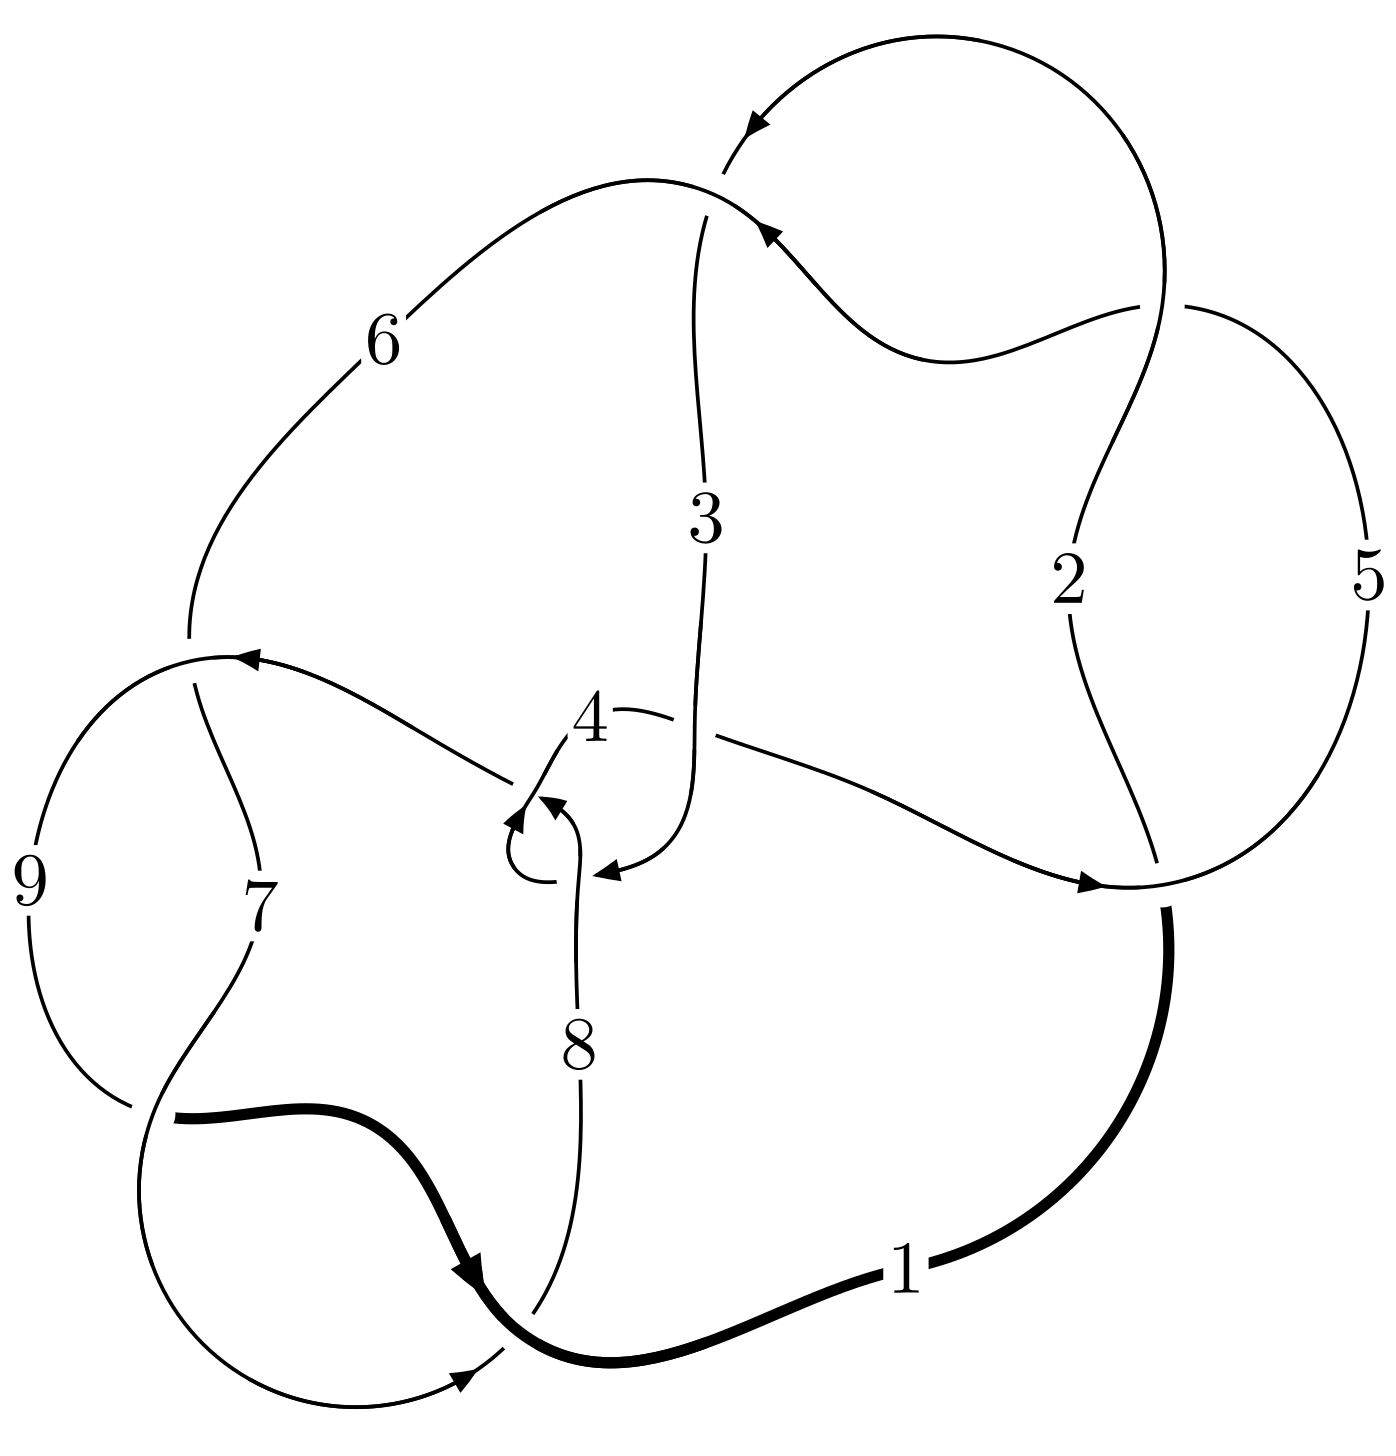
\includegraphics[width=112pt]{../../../GIT/diagram.site/Diagrams/png/51_9_16.png}\\
\ \ \ A knot diagram\footnotemark}&
\allowdisplaybreaks
\textbf{Linearized knot diagam} \\
\cline{2-2}
 &
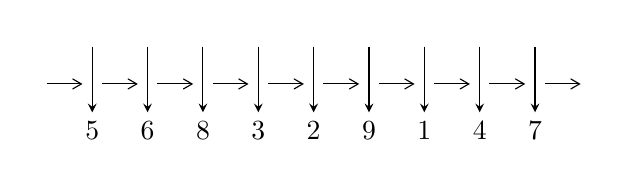
\begin{tikzpicture}[x=20pt, y=17pt]
	% nodes
	\node (C0) at (0, 0) {};
	\node (C1) at (1, 0) {};
	\node (C1U) at (1, +1) {};
	\node (C1D) at (1, -1) {5};

	\node (C2) at (2, 0) {};
	\node (C2U) at (2, +1) {};
	\node (C2D) at (2, -1) {6};

	\node (C3) at (3, 0) {};
	\node (C3U) at (3, +1) {};
	\node (C3D) at (3, -1) {8};

	\node (C4) at (4, 0) {};
	\node (C4U) at (4, +1) {};
	\node (C4D) at (4, -1) {3};

	\node (C5) at (5, 0) {};
	\node (C5U) at (5, +1) {};
	\node (C5D) at (5, -1) {2};

	\node (C6) at (6, 0) {};
	\node (C6U) at (6, +1) {};
	\node (C6D) at (6, -1) {9};

	\node (C7) at (7, 0) {};
	\node (C7U) at (7, +1) {};
	\node (C7D) at (7, -1) {1};

	\node (C8) at (8, 0) {};
	\node (C8U) at (8, +1) {};
	\node (C8D) at (8, -1) {4};

	\node (C9) at (9, 0) {};
	\node (C9U) at (9, +1) {};
	\node (C9D) at (9, -1) {7};
	\node (C10) at (10, 0) {};

	% arrows
	\draw[->,>={angle 60}]
	(C0) edge (C1) (C1) edge (C2) (C2) edge (C3) (C3) edge (C4) (C4) edge (C5) (C5) edge (C6) (C6) edge (C7) (C7) edge (C8) (C8) edge (C9) (C9) edge (C10) ;	\draw[->,>=stealth]
	(C1U) edge (C1D) (C2U) edge (C2D) (C3U) edge (C3D) (C4U) edge (C4D) (C5U) edge (C5D) (C6U) edge (C6D) (C7U) edge (C7D) (C8U) edge (C8D) (C9U) edge (C9D) ;
	\end{tikzpicture} \\
\hhline{~~} \\& 
\textbf{Solving Sequence} \\ \cline{2-2} 
 &
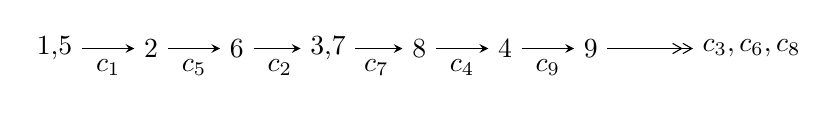
\begin{tikzpicture}[x=31pt, y=7pt]
	% node
	\node (A0) at (-1/8, 0) {1,5};
	\node (A1) at (1, 0) {2};
	\node (A2) at (2, 0) {6};
	\node (A3) at (49/16, 0) {3,7};
	\node (A4) at (33/8, 0) {8};
	\node (A5) at (41/8, 0) {4};
	\node (A6) at (49/8, 0) {9};
	\node (C1) at (1/2, -1) {$c_{1}$};
	\node (C2) at (3/2, -1) {$c_{5}$};
	\node (C3) at (5/2, -1) {$c_{2}$};
	\node (C4) at (29/8, -1) {$c_{7}$};
	\node (C5) at (37/8, -1) {$c_{4}$};
	\node (C6) at (45/8, -1) {$c_{9}$};
	\node (A7) at (8, 0) {$c_{3},c_{6},c_{8}$};

	% edge
	\draw[->,>=stealth]	
	(A0) edge (A1) (A1) edge (A2) (A2) edge (A3) (A3) edge (A4) (A4) edge (A5) (A5) edge (A6) ;
	\draw[->>,>={angle 60}]	
	(A6) edge (A7);
\end{tikzpicture} \\ 

\end{tabular} \\

\footnotetext{
The image of knot diagram is generated by the software ``\textbf{Draw programme}" developed by Andrew Bartholomew(\url{http://www.layer8.co.uk/maths/draw/index.htm\#Running-draw}), where we modified some parts for our purpose(\url{https://github.com/CATsTAILs/LinksPainter}).
}\phantom \\ \newline 
\centering \textbf{Ideals for irreducible components\footnotemark of $X_{\text{par}}$} 
 
\begin{align*}
I^u_{1}&=\langle 
b- u,\;u^6+u^5-3 u^4-2 u^3+2 u^2+a- u+1,\;u^8+u^7-4 u^6-3 u^5+5 u^4+u^3- u^2+3 u-1\rangle \\
I^u_{2}&=\langle 
- u^{11}+4 u^9- u^8-5 u^7+3 u^6+u^5-2 u^4+u^3+b+u-1,\\
\phantom{I^u_{2}}&\phantom{= \langle  }- u^{11}- u^{10}+4 u^9+2 u^8-7 u^7+u^6+5 u^5-5 u^4+u^3+3 u^2+a-2 u,\\
\phantom{I^u_{2}}&\phantom{= \langle  }u^{12}+u^{11}-4 u^{10}-2 u^9+7 u^8- u^7-5 u^6+5 u^5- u^4-3 u^3+2 u^2+1\rangle \\
I^u_{3}&=\langle 
b+1,\;a+1,\;u-1\rangle \\
\\
\end{align*}
\raggedright * 3 irreducible components of $\dim_{\mathbb{C}}=0$, with total 21 representations.\\
\footnotetext{All coefficients of polynomials are rational numbers. But the coefficients are sometimes approximated in decimal forms when there is not enough margin.}
\newpage
\renewcommand{\arraystretch}{1}
\centering \section*{I. $I^u_{1}= \langle b- u,\;u^6+u^5-3 u^4-2 u^3+2 u^2+a- u+1,\;u^8+u^7-4 u^6-3 u^5+5 u^4+u^3- u^2+3 u-1 \rangle$}
\flushleft \textbf{(i) Arc colorings}\\
\begin{tabular}{m{7pt} m{180pt} m{7pt} m{180pt} }
\flushright $a_{1}=$&$\begin{pmatrix}1\\0\end{pmatrix}$ \\
\flushright $a_{5}=$&$\begin{pmatrix}0\\u\end{pmatrix}$ \\
\flushright $a_{2}=$&$\begin{pmatrix}1\\u^2\end{pmatrix}$ \\
\flushright $a_{6}=$&$\begin{pmatrix}- u\\- u^3+u\end{pmatrix}$ \\
\flushright $a_{3}=$&$\begin{pmatrix}- u^2+1\\- u^4+2 u^2\end{pmatrix}$ \\
\flushright $a_{7}=$&$\begin{pmatrix}- u^6- u^5+3 u^4+2 u^3-2 u^2+u-1\\u\end{pmatrix}$ \\
\flushright $a_{8}=$&$\begin{pmatrix}- u^6- u^5+3 u^4+2 u^3-2 u^2-1\\u\end{pmatrix}$ \\
\flushright $a_{4}=$&$\begin{pmatrix}u^5-2 u^3+u\\u^7-3 u^5+2 u^3+u\end{pmatrix}$ \\
\flushright $a_{9}=$&$\begin{pmatrix}u^7+u^6-3 u^5-2 u^4+2 u^3- u^2+u+1\\- u^2\end{pmatrix}$\\ \flushright $a_{9}=$&$\begin{pmatrix}u^7+u^6-3 u^5-2 u^4+2 u^3- u^2+u+1\\- u^2\end{pmatrix}$\\&\end{tabular}
\flushleft \textbf{(ii) Obstruction class $= -1$}\\~\\
\flushleft \textbf{(iii) Cusp Shapes $= -2 u^6+2 u^5+10 u^4-8 u^3-12 u^2+10 u-16$}\\~\\
\newpage\renewcommand{\arraystretch}{1}
\flushleft \textbf{(iv) u-Polynomials at the component}\newline \\
\begin{tabular}{m{50pt}|m{274pt}}
Crossings & \hspace{64pt}u-Polynomials at each crossing \\
\hline $$\begin{aligned}c_{1},c_{2},c_{5}\\c_{6},c_{7},c_{9}\end{aligned}$$&$\begin{aligned}
&u^8- u^7-4 u^6+3 u^5+5 u^4- u^3- u^2-3 u-1
\end{aligned}$\\
\hline $$\begin{aligned}c_{3},c_{8}\end{aligned}$$&$\begin{aligned}
&u^8-3 u^7+3 u^6+2 u^5-8 u^4+9 u^3-3 u^2-2 u+2
\end{aligned}$\\
\hline $$\begin{aligned}c_{4}\end{aligned}$$&$\begin{aligned}
&u^8+3 u^7+5 u^6+4 u^5+2 u^4+13 u^3+13 u^2+16 u+4
\end{aligned}$\\
\hline
\end{tabular}\\~\\
\newpage\renewcommand{\arraystretch}{1}
\flushleft \textbf{(v) Riley Polynomials at the component}\newline \\
\begin{tabular}{m{50pt}|m{274pt}}
Crossings & \hspace{64pt}Riley Polynomials at each crossing \\
\hline $$\begin{aligned}c_{1},c_{2},c_{5}\\c_{6},c_{7},c_{9}\end{aligned}$$&$\begin{aligned}
&y^8-9 y^7+32 y^6-53 y^5+31 y^4+15 y^3-15 y^2-7 y+1
\end{aligned}$\\
\hline $$\begin{aligned}c_{3},c_{8}\end{aligned}$$&$\begin{aligned}
&y^8-3 y^7+5 y^6-4 y^5+2 y^4-13 y^3+13 y^2-16 y+4
\end{aligned}$\\
\hline $$\begin{aligned}c_{4}\end{aligned}$$&$\begin{aligned}
&y^8+y^7+5 y^6-48 y^5-58 y^4-205 y^3-231 y^2-152 y+16
\end{aligned}$\\
\hline
\end{tabular}\\~\\
\newpage\flushleft \textbf{(vi) Complex Volumes and Cusp Shapes}
$$\begin{array}{c|c|c}  
\text{Solutions to }I^u_{1}& \I (\text{vol} + \sqrt{-1}CS) & \text{Cusp shape}\\
 \hline 
\begin{aligned}
u &= \phantom{-}0.151337 + 0.673064 I \\
a &= -0.076017 - 0.952103 I \\
b &= \phantom{-}0.151337 + 0.673064 I\end{aligned}
 & \phantom{-}1.48505 - 2.26376 I & -5.94128 + 4.53378 I \\ \hline\begin{aligned}
u &= \phantom{-}0.151337 - 0.673064 I \\
a &= -0.076017 + 0.952103 I \\
b &= \phantom{-}0.151337 - 0.673064 I\end{aligned}
 & \phantom{-}1.48505 + 2.26376 I & -5.94128 - 4.53378 I \\ \hline\begin{aligned}
u &= \phantom{-}1.359440 + 0.207304 I \\
a &= \phantom{-}2.50827 - 1.24101 I \\
b &= \phantom{-}1.359440 + 0.207304 I\end{aligned}
 & -6.22518 - 3.55755 I & -14.5274 + 2.6249 I \\ \hline\begin{aligned}
u &= \phantom{-}1.359440 - 0.207304 I \\
a &= \phantom{-}2.50827 + 1.24101 I \\
b &= \phantom{-}1.359440 - 0.207304 I\end{aligned}
 & -6.22518 + 3.55755 I & -14.5274 - 2.6249 I \\ \hline\begin{aligned}
u &= -1.42757 + 0.33227 I \\
a &= -1.86256 - 1.18850 I \\
b &= -1.42757 + 0.33227 I\end{aligned}
 & -8.73978 + 9.88301 I & -15.2825 - 6.0696 I \\ \hline\begin{aligned}
u &= -1.42757 - 0.33227 I \\
a &= -1.86256 + 1.18850 I \\
b &= -1.42757 - 0.33227 I\end{aligned}
 & -8.73978 - 9.88301 I & -15.2825 + 6.0696 I \\ \hline\begin{aligned}
u &= -1.50912\phantom{ +0.000000I} \\
a &= -2.36273\phantom{ +0.000000I} \\
b &= -1.50912\phantom{ +0.000000I}\end{aligned}
 & -13.4445\phantom{ +0.000000I} & -18.3370\phantom{ +0.000000I} \\ \hline\begin{aligned}
u &= \phantom{-}0.342714\phantom{ +0.000000I} \\
a &= -0.776649\phantom{ +0.000000I} \\
b &= \phantom{-}0.342714\phantom{ +0.000000I}\end{aligned}
 & -0.719034\phantom{ +0.000000I} & -14.1600\phantom{ +0.000000I}\\
 \hline 
 \end{array}$$\newpage\newpage\renewcommand{\arraystretch}{1}
\centering \section*{II. $I^u_{2}= \langle - u^{11}+4 u^9+\cdots+b-1,\;- u^{11}- u^{10}+\cdots+a-2 u,\;u^{12}+u^{11}+\cdots+2 u^2+1 \rangle$}
\flushleft \textbf{(i) Arc colorings}\\
\begin{tabular}{m{7pt} m{180pt} m{7pt} m{180pt} }
\flushright $a_{1}=$&$\begin{pmatrix}1\\0\end{pmatrix}$ \\
\flushright $a_{5}=$&$\begin{pmatrix}0\\u\end{pmatrix}$ \\
\flushright $a_{2}=$&$\begin{pmatrix}1\\u^2\end{pmatrix}$ \\
\flushright $a_{6}=$&$\begin{pmatrix}- u\\- u^3+u\end{pmatrix}$ \\
\flushright $a_{3}=$&$\begin{pmatrix}- u^2+1\\- u^4+2 u^2\end{pmatrix}$ \\
\flushright $a_{7}=$&$\begin{pmatrix}u^{11}+u^{10}-4 u^9-2 u^8+7 u^7- u^6-5 u^5+5 u^4- u^3-3 u^2+2 u\\u^{11}-4 u^9+u^8+5 u^7-3 u^6- u^5+2 u^4- u^3- u+1\end{pmatrix}$ \\
\flushright $a_{8}=$&$\begin{pmatrix}u^{10}-3 u^8+2 u^7+2 u^6-4 u^5+3 u^4-3 u^2+3 u-1\\u^{11}-4 u^9+u^8+5 u^7-3 u^6- u^5+2 u^4- u^3- u+1\end{pmatrix}$ \\
\flushright $a_{4}=$&$\begin{pmatrix}u^5-2 u^3+u\\u^7-3 u^5+2 u^3+u\end{pmatrix}$ \\
\flushright $a_{9}=$&$\begin{pmatrix}- u^{11}+4 u^9-2 u^8-6 u^7+6 u^6+2 u^5-6 u^4+3 u^3+2 u^2-2 u\\- u^{11}+3 u^9-2 u^8-2 u^7+4 u^6-3 u^5+3 u^3-2 u^2+u-2\end{pmatrix}$\\ \flushright $a_{9}=$&$\begin{pmatrix}- u^{11}+4 u^9-2 u^8-6 u^7+6 u^6+2 u^5-6 u^4+3 u^3+2 u^2-2 u\\- u^{11}+3 u^9-2 u^8-2 u^7+4 u^6-3 u^5+3 u^3-2 u^2+u-2\end{pmatrix}$\\&\end{tabular}
\flushleft \textbf{(ii) Obstruction class $= -1$}\\~\\
\flushleft \textbf{(iii) Cusp Shapes $= -4 u^8+12 u^6-4 u^5-8 u^4+8 u^3-4 u^2-10$}\\~\\
\newpage\renewcommand{\arraystretch}{1}
\flushleft \textbf{(iv) u-Polynomials at the component}\newline \\
\begin{tabular}{m{50pt}|m{274pt}}
Crossings & \hspace{64pt}u-Polynomials at each crossing \\
\hline $$\begin{aligned}c_{1},c_{2},c_{5}\\c_{6},c_{7},c_{9}\end{aligned}$$&$\begin{aligned}
&u^{12}- u^{11}-4 u^{10}+2 u^9+7 u^8+u^7-5 u^6-5 u^5- u^4+3 u^3+2 u^2+1
\end{aligned}$\\
\hline $$\begin{aligned}c_{3},c_{8}\end{aligned}$$&$\begin{aligned}
&(u^6+u^5- u^4-2 u^3+u+1)^2
\end{aligned}$\\
\hline $$\begin{aligned}c_{4}\end{aligned}$$&$\begin{aligned}
&(u^6+3 u^5+5 u^4+4 u^3+2 u^2+u+1)^2
\end{aligned}$\\
\hline
\end{tabular}\\~\\
\newpage\renewcommand{\arraystretch}{1}
\flushleft \textbf{(v) Riley Polynomials at the component}\newline \\
\begin{tabular}{m{50pt}|m{274pt}}
Crossings & \hspace{64pt}Riley Polynomials at each crossing \\
\hline $$\begin{aligned}c_{1},c_{2},c_{5}\\c_{6},c_{7},c_{9}\end{aligned}$$&$\begin{aligned}
&y^{12}-9 y^{11}+\cdots+4 y+1
\end{aligned}$\\
\hline $$\begin{aligned}c_{3},c_{8}\end{aligned}$$&$\begin{aligned}
&(y^6-3 y^5+5 y^4-4 y^3+2 y^2- y+1)^2
\end{aligned}$\\
\hline $$\begin{aligned}c_{4}\end{aligned}$$&$\begin{aligned}
&(y^6+y^5+5 y^4+6 y^2+3 y+1)^2
\end{aligned}$\\
\hline
\end{tabular}\\~\\
\newpage\flushleft \textbf{(vi) Complex Volumes and Cusp Shapes}
$$\begin{array}{c|c|c}  
\text{Solutions to }I^u_{2}& \I (\text{vol} + \sqrt{-1}CS) & \text{Cusp shape}\\
 \hline 
\begin{aligned}
u &= \phantom{-}0.895235 + 0.524661 I \\
a &= -0.831450 + 0.487279 I \\
b &= -1.323480 + 0.139870 I\end{aligned}
 & -5.18047 + 0.92430 I & -15.7167 - 0.7942 I \\ \hline\begin{aligned}
u &= \phantom{-}0.895235 - 0.524661 I \\
a &= -0.831450 - 0.487279 I \\
b &= -1.323480 - 0.139870 I\end{aligned}
 & -5.18047 - 0.92430 I & -15.7167 + 0.7942 I \\ \hline\begin{aligned}
u &= \phantom{-}0.282166 + 0.828798 I \\
a &= -0.368111 + 1.081240 I \\
b &= -1.356120 - 0.270046 I\end{aligned}
 & -3.28987 - 5.69302 I & -12.00000 + 5.51057 I \\ \hline\begin{aligned}
u &= \phantom{-}0.282166 - 0.828798 I \\
a &= -0.368111 - 1.081240 I \\
b &= -1.356120 + 0.270046 I\end{aligned}
 & -3.28987 + 5.69302 I & -12.00000 - 5.51057 I \\ \hline\begin{aligned}
u &= \phantom{-}1.155020 + 0.191936 I \\
a &= -0.842520 + 0.140006 I \\
b &= -0.152828 - 0.487477 I\end{aligned}
 & -1.39926 - 0.92430 I & -8.28328 + 0.79423 I \\ \hline\begin{aligned}
u &= \phantom{-}1.155020 - 0.191936 I \\
a &= -0.842520 - 0.140006 I \\
b &= -0.152828 + 0.487477 I\end{aligned}
 & -1.39926 + 0.92430 I & -8.28328 - 0.79423 I \\ \hline\begin{aligned}
u &= -1.323480 + 0.139870 I \\
a &= \phantom{-}0.747239 + 0.078971 I \\
b &= \phantom{-}0.895235 + 0.524661 I\end{aligned}
 & -5.18047 + 0.92430 I & -15.7167 - 0.7942 I \\ \hline\begin{aligned}
u &= -1.323480 - 0.139870 I \\
a &= \phantom{-}0.747239 - 0.078971 I \\
b &= \phantom{-}0.895235 - 0.524661 I\end{aligned}
 & -5.18047 - 0.92430 I & -15.7167 + 0.7942 I \\ \hline\begin{aligned}
u &= -1.356120 + 0.270046 I \\
a &= \phantom{-}0.709275 + 0.141239 I \\
b &= \phantom{-}0.282166 - 0.828798 I\end{aligned}
 & -3.28987 + 5.69302 I & -12.00000 - 5.51057 I \\ \hline\begin{aligned}
u &= -1.356120 - 0.270046 I \\
a &= \phantom{-}0.709275 - 0.141239 I \\
b &= \phantom{-}0.282166 + 0.828798 I\end{aligned}
 & -3.28987 - 5.69302 I & -12.00000 + 5.51057 I\\
 \hline 
 \end{array}$$\newpage$$\begin{array}{c|c|c}  
\text{Solutions to }I^u_{2}& \I (\text{vol} + \sqrt{-1}CS) & \text{Cusp shape}\\
 \hline 
\begin{aligned}
u &= -0.152828 + 0.487477 I \\
a &= \phantom{-}0.58557 + 1.86780 I \\
b &= \phantom{-}1.155020 - 0.191936 I\end{aligned}
 & -1.39926 + 0.92430 I & -8.28328 - 0.79423 I \\ \hline\begin{aligned}
u &= -0.152828 - 0.487477 I \\
a &= \phantom{-}0.58557 - 1.86780 I \\
b &= \phantom{-}1.155020 + 0.191936 I\end{aligned}
 & -1.39926 - 0.92430 I & -8.28328 + 0.79423 I\\
 \hline 
 \end{array}$$\newpage\newpage\renewcommand{\arraystretch}{1}
\centering \section*{III. $I^u_{3}= \langle b+1,\;a+1,\;u-1 \rangle$}
\flushleft \textbf{(i) Arc colorings}\\
\begin{tabular}{m{7pt} m{180pt} m{7pt} m{180pt} }
\flushright $a_{1}=$&$\begin{pmatrix}1\\0\end{pmatrix}$ \\
\flushright $a_{5}=$&$\begin{pmatrix}0\\1\end{pmatrix}$ \\
\flushright $a_{2}=$&$\begin{pmatrix}1\\1\end{pmatrix}$ \\
\flushright $a_{6}=$&$\begin{pmatrix}-1\\0\end{pmatrix}$ \\
\flushright $a_{3}=$&$\begin{pmatrix}0\\1\end{pmatrix}$ \\
\flushright $a_{7}=$&$\begin{pmatrix}-1\\-1\end{pmatrix}$ \\
\flushright $a_{8}=$&$\begin{pmatrix}0\\-1\end{pmatrix}$ \\
\flushright $a_{4}=$&$\begin{pmatrix}0\\1\end{pmatrix}$ \\
\flushright $a_{9}=$&$\begin{pmatrix}0\\-1\end{pmatrix}$\\ \flushright $a_{9}=$&$\begin{pmatrix}0\\-1\end{pmatrix}$\\&\end{tabular}
\flushleft \textbf{(ii) Obstruction class $= 1$}\\~\\
\flushleft \textbf{(iii) Cusp Shapes $= -12$}\\~\\
\newpage\renewcommand{\arraystretch}{1}
\flushleft \textbf{(iv) u-Polynomials at the component}\newline \\
\begin{tabular}{m{50pt}|m{274pt}}
Crossings & \hspace{64pt}u-Polynomials at each crossing \\
\hline $$\begin{aligned}c_{1},c_{2},c_{6}\\c_{7}\end{aligned}$$&$\begin{aligned}
&u-1
\end{aligned}$\\
\hline $$\begin{aligned}c_{3},c_{4},c_{8}\end{aligned}$$&$\begin{aligned}
&u
\end{aligned}$\\
\hline $$\begin{aligned}c_{5},c_{9}\end{aligned}$$&$\begin{aligned}
&u+1
\end{aligned}$\\
\hline
\end{tabular}\\~\\
\newpage\renewcommand{\arraystretch}{1}
\flushleft \textbf{(v) Riley Polynomials at the component}\newline \\
\begin{tabular}{m{50pt}|m{274pt}}
Crossings & \hspace{64pt}Riley Polynomials at each crossing \\
\hline $$\begin{aligned}c_{1},c_{2},c_{5}\\c_{6},c_{7},c_{9}\end{aligned}$$&$\begin{aligned}
&y-1
\end{aligned}$\\
\hline $$\begin{aligned}c_{3},c_{4},c_{8}\end{aligned}$$&$\begin{aligned}
&y
\end{aligned}$\\
\hline
\end{tabular}\\~\\
\newpage\flushleft \textbf{(vi) Complex Volumes and Cusp Shapes}
$$\begin{array}{c|c|c}  
\text{Solutions to }I^u_{3}& \I (\text{vol} + \sqrt{-1}CS) & \text{Cusp shape}\\
 \hline 
\begin{aligned}
u &= \phantom{-}1.00000\phantom{ +0.000000I} \\
a &= -1.00000\phantom{ +0.000000I} \\
b &= -1.00000\phantom{ +0.000000I}\end{aligned}
 & -3.28987\phantom{ +0.000000I} & -12.0000\phantom{ +0.000000I}\\
 \hline 
 \end{array}$$\newpage
\newpage\renewcommand{\arraystretch}{1}
\centering \section*{ IV. u-Polynomials}
\begin{tabular}{m{50pt}|m{274pt}}
Crossings & \hspace{64pt}u-Polynomials at each crossing \\
\hline $$\begin{aligned}c_{1},c_{2},c_{6}\\c_{7}\end{aligned}$$&$\begin{aligned}
&(u-1)(u^8- u^7-4 u^6+3 u^5+5 u^4- u^3- u^2-3 u-1)\\
&\cdot(u^{12}- u^{11}-4 u^{10}+2 u^9+7 u^8+u^7-5 u^6-5 u^5- u^4+3 u^3+2 u^2+1)
\end{aligned}$\\
\hline $$\begin{aligned}c_{3},c_{8}\end{aligned}$$&$\begin{aligned}
&u(u^6+u^5- u^4-2 u^3+u+1)^2\\
&\cdot(u^8-3 u^7+3 u^6+2 u^5-8 u^4+9 u^3-3 u^2-2 u+2)
\end{aligned}$\\
\hline $$\begin{aligned}c_{4}\end{aligned}$$&$\begin{aligned}
&u(u^6+3 u^5+5 u^4+4 u^3+2 u^2+u+1)^2\\
&\cdot(u^8+3 u^7+5 u^6+4 u^5+2 u^4+13 u^3+13 u^2+16 u+4)
\end{aligned}$\\
\hline $$\begin{aligned}c_{5},c_{9}\end{aligned}$$&$\begin{aligned}
&(u+1)(u^8- u^7-4 u^6+3 u^5+5 u^4- u^3- u^2-3 u-1)\\
&\cdot(u^{12}- u^{11}-4 u^{10}+2 u^9+7 u^8+u^7-5 u^6-5 u^5- u^4+3 u^3+2 u^2+1)
\end{aligned}$\\
\hline
\end{tabular}\newpage\renewcommand{\arraystretch}{1}
\centering \section*{ V. Riley Polynomials}
\begin{tabular}{m{50pt}|m{274pt}}
Crossings & \hspace{64pt}Riley Polynomials at each crossing \\
\hline $$\begin{aligned}c_{1},c_{2},c_{5}\\c_{6},c_{7},c_{9}\end{aligned}$$&$\begin{aligned}
&(y-1)(y^8-9 y^7+32 y^6-53 y^5+31 y^4+15 y^3-15 y^2-7 y+1)\\
&\cdot(y^{12}-9 y^{11}+\cdots+4 y+1)
\end{aligned}$\\
\hline $$\begin{aligned}c_{3},c_{8}\end{aligned}$$&$\begin{aligned}
&y(y^6-3 y^5+5 y^4-4 y^3+2 y^2- y+1)^2\\
&\cdot(y^8-3 y^7+5 y^6-4 y^5+2 y^4-13 y^3+13 y^2-16 y+4)
\end{aligned}$\\
\hline $$\begin{aligned}c_{4}\end{aligned}$$&$\begin{aligned}
&y(y^6+y^5+5 y^4+6 y^2+3 y+1)^2\\
&\cdot(y^8+y^7+5 y^6-48 y^5-58 y^4-205 y^3-231 y^2-152 y+16)
\end{aligned}$\\
\hline
\end{tabular}
\vskip 2pc
\end{document}